\documentclass[11pt,onecolumn]{article}
\usepackage{amsmath,amssymb,graphicx,algorithmic,xspace,url}
\usepackage[titlenotnumbered,noend,noline]{algorithm2e}
\usepackage{enumerate}
\usepackage{mathrsfs}
\usepackage{array}

\setlength{\pdfpagewidth}{8.5in}
\setlength{\pdfpageheight}{11in}
\setlength{\evensidemargin}{-0.1in} \setlength{\oddsidemargin}{-0.1in}
\setlength{\textwidth}{6.5in} \setlength{\textheight}{9.0in}
\setlength{\topmargin}{-0.6in}

\sloppypar
\begin{document}

\begin{center}
\begin{Large}
ECE 493, Spring 2020, Assignment 1\\
Due: Friday June 19, 11:59pm
\end{Large}
\end{center}
\vspace{.2em}

\vspace{.2em}
\begin{center}
Submit to the UWaterloo Crowdmark site using the link you received via email.
Your answer can be handwritten converted to an electronic file by and scanner or camera; or the answers can be typed up in a word processor or LaTeX and submitted as a pdf.
\end{center}
\vspace{.2em}

\vspace{.2em}


\section{Basics of Probability}

\begin{enumerate}
    \item Let $X$ and $Y$ be two random variables. If $X$ and $Y$ are uncorrelated, does it imply $X$ and $Y$ are independent? If yes, show how, else provide a counterexample. 
    
    \item A satellite is sending a binary message/code, i.e.\ a sequence of 1s and 0s. Suppose 70\% of the message to be sent is 0s. There is a 80\% chance of a given 0 or 1 being received correctly. Find the probability that 0 was sent if 1 was received. 
    
    \item \textbf{Basic Inference}: The probability of getting a headache is $1/10$, getting the flu is $1/40$, and if you have a flu, there's $1/2$ chance of getting the headache. One day you wake up with a headache and say `Dang, I have a headache. Since 50\% of flues are associated with headaches, I must have a 50-50 chance of coming down with the flu'. Is this line of reasoning correct? Why/Why not? 

    \item \textbf{Bayesian Learning}: We are interested in forming a belief (hypothesis) about our environment based on what we have observed (evidence). Bayes rule is important when we want to assign a probability to our hypothesis after observing some evidence. Recall Bayes Rule:
    
    \begin{equation*}
        \mathbb{P}(H|e) = \frac{\mathbb{P}(e|H) \mathbb{P}(H)}{\mathbb{P}(e)},
    \end{equation*}
    where $H$ is the hypothesis, $e$ is the evidence, $\mathbb{P}(H)$ is our prior distribution over the different hypotheses, $\mathbb{P}(e|H)$ is the likelihood of the evidence given our hypothesis, $\mathbb{P}(H|e)$ is the posterior distribution of the different hypotheses given the evidence, and $\mathbb{P}(e)$ is the probability of the evidence.
    
    Suppose there are five kinds of bags of marbles: 
    \begin{enumerate}
        \item 10\% are bags of type $h_1$ with 100\% red marbles.
        \item 20\% are bags of type $h_2$ with 75\% red marbles and 25\% green marbles.
        \item 40\% are bags of type $h_3$ with 50\% red marbles and 50\% green marbles.
        \item 20\% are bags of type $h_4$ with 25\% red marbles and 75\% green marbles.
        \item 10\% are bags of type $h_5$ with 100\% green marbles.
    \end{enumerate}
    
    We buy a bag at random, pick 5 marbles from the bag and observe them to be all green. We are interested in knowing what type of bag we bought and what colour the next marble will be. 
    
    Let $e$ be the event that the 5 marbles drawn are green and let $\mathbb{P}(e) = \alpha$. 
    
    \begin{enumerate}
        \item Given that the 5 marbles drawn were green, compute the probability of each type of bag i.e.\ what is the probability of bag type $h_i$ for $i = \{1, 2, 3, 4, 5\}$, given that 5 marbles picked were green?
        
        \item Use the results from part (a) to find the value of $\alpha$ using the axioms of probability.
        
        \item Let $X$ be a random variable that represents the outcome of the next pick from the bag i.e.\ $X$ can be either green or red. How would you make a prediction about the outcome of $X$, given that the first 5 marbles picked were green? (Give an equation for $\mathbb{P}(X|e)$) Hint: Think about how you can use the concept of joint and marginal distributions with the events of picking different types of bags.
        
        \item Use the result from part (c) to compute $\mathbb{P}(X=\text{"green"} |e)$.
        
    \end{enumerate}
\end{enumerate} 


\section{Multi-Armed Bandits}
\begin{enumerate}
    \item Consider a k-armed bandit problem with k = 4 actions, denoted 1, 2, 3, and 4. Consider applying to this problem a bandit algorithm using $\epsilon$-greedy action selection, sample-average action-value estimates, and initial estimates of Q1(a) = 0, for all a. Suppose the initial sequence of actions and rewards is $A_1$ = 1, $R_1$ = 1, $A_2$ = 2, $R_2$ = 1, $A_3$ = 2, $R_3$ = 2, $A_4$ = 2, $R_4$ = 2, $A_5$ = 3, $R_5$ = 0. On some of these time steps the $\epsilon$ case may have occurred, causing an action to be selected at random. On which time steps did this definitely occur? On which time steps could this possibly have occurred? 
    
    \item Suppose you face a 2-armed bandit task whose true action values change randomly from time step to time step. Specifically, suppose that, for any time step, the true values of actions 1 and 2 are respectively 10 and 20 with probability 0.5 (case A), and 90 and 80 with probability 0.5 (case B). If you are not able to tell which case you face at any step, what is the best expected reward you can achieve and how should you behave to achieve it? Now suppose that on each step you are told whether you are facing case A or case B (although you still don’t know the true action values). This is an associative search task. What is the best expected reward you can achieve in this task, and how should you behave to achieve it?
\end{enumerate}



\section{MDPs}

\begin{enumerate}
    \item Let $G_t = R_{t+1} + \gamma R_{t+2} + \ldots + \gamma^{T-1} R_{T}$. Suppose $\gamma = 0.5$ and the following sequence of rewards is received: $R_1$ = 1, $R_2$ = 2, $R_3$ = 5, $R_4$ = -2, $R_5$ = 2, and $T$ = 5. Solve for $G_0$, $G_1$, $G_2$, $G_3$, $G_4$, and $G_5$.
    
    \item Let $G_t = \sum_{k=0}^\infty \gamma^k R_{t+k+1}$. Suppose $\gamma = 0.9$ and the reward sequence is $R_1 =2$, followed by an infinite sequence of 6s. What are $G_0$ and $G_1$?
    
    \item Suppose you treated pole-balancing as an episodic task but also used discounting, with all rewards zero except for -1 upon failure. What then would the return be at each time? How does this return differ from that in the discounted, continuing formulation of this task? (For explanation of pole-balancing see Example 3.4 on Sutton's RL Book)
    
    \item Figure \ref{fig:book3.14} (left) shows a rectangular grid world representation of a simple finite MDP. The cells of the grid correspond to the states of the environment. At each cell, four actions are possible: north, south, east, and west, which deterministically cause the agent to move one cell in the respective direction on the grid. Actions that would take the agent off the grid leave its location unchanged, but also result in a reward of -1. Other actions result in a reward of 0, except those that move the agent out of the special states A and B. From state A, all four actions yield a reward of +10 and take the agent to A'. From state B, all actions yield a reward of +5 and take the agent to B'. 
    
    Assuming discount factor $\gamma=0.9$ and equal probabilities to all four actions, value functions seen in Figure \ref{fig:book3.14} (right) obtained. Show numerically that the Bellman expectation equation holds for the cell at the middle of top row, valued at +4.4, with respect to its four neighboring states, valued at +8.8, +2.3, +5.3 and off-grid (These numbers are accurate only to one decimal place.) (\textbf{Hint:} Try to understand what happens when agent takes action to north, off-grid)
    
\end{enumerate}

\begin{figure}[htbp]
    \centering
    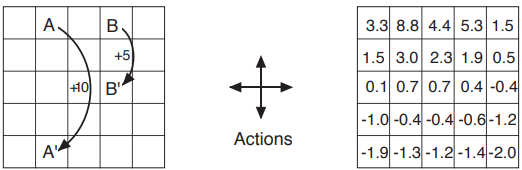
\includegraphics[width=0.6\linewidth]{figures/mdp_grid.png}
    
    \caption{Gridworld example: exceptional reward dynamics (left) and state-value function for the equiprobable random policy (right)}
    \label{fig:book3.14}
\end{figure}


\end{document}
